\documentclass[12pt,a4paper]{article}

% Basic packages
\usepackage[utf8]{inputenc}
\usepackage[T1]{fontenc}
\usepackage{amsmath,amssymb,amsfonts}
\usepackage{graphicx}
\usepackage{hyperref}
\usepackage{geometry}
\usepackage{pgfplots}
\pgfplotsset{compat=1.18}

% Set margins
\geometry{margin=1in}

% Document info
\title{AI 1.1: The Neuron and Backpropagation}
\author{Tavish Mankash}
\date{}

\begin{document}

\maketitle

\section{The Neuron}
\begin{figure}[ht]
    \centering
    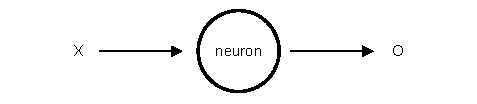
\includegraphics[width=0.9\textwidth]{../figs/Neuron.drawio.pdf}
    \caption{Diagram of a neuron}
    \label{fig:neuron}
\end{figure}

A neuron is a cell in the human brain that transmits information through electrical and chemical signals. We will model it mathematically as a function that takes inputs and produces an output.

\[
Y = WX + B
\]

where:
\[
\begin{aligned}
    Y & : \text{Output of the neuron} \\
    W & : \text{Weight of the neuron} \\
    X & : \text{Inputs to the neuron} \\
    B & : \text{Bias of the neuron}
\end{aligned}
\]

\subsection{Example}
\begin{table}[ht]
    \centering
    \begin{tabular}{|c|c|}
        \hline
        $X$ & $\hat{Y}$ \\ \hline
        4   & 8         \\ \hline
    \end{tabular}
    \caption{Example values of $X$ and $\hat{Y}$ for modeling a 2x function}
    \label{tab:example}
\end{table}


$\hat{Y}$ is the ideal output of the neuron.
The following are ideal values for $W$ and $B$:
W=2, B=0

The objective of AI algorithms is to find the best values of $W$ and $B$ such that the output of the neuron is as close to $\hat{Y}$ as possible.

\section{Backpropagation}
Backpropagation is the fundamental algorithm used to train neural networks. It essentially works by figuring out how much each weight and bias contributed to the overall loss, and then adjusting them in a way that minimizes this loss. We'll explore the concepts behind this process.

\subsection{Manual Weight and Bias Adjustment}
We initialize the values of $W$ and $B$ randomly. We then calculate the output of the neuron using the formula above. We then calculate the loss L between the output and the ideal output $\hat{Y}$ using the following formula:
\[
L =
(Y - \hat{Y})^2\]
Loss represents how far away our current output is from the ideal answer ($\hat{Y}$), and it is a value we aim to minimize through training.
The loss is squared to make it positive. Additionally, it penalizes large losses significantly while minimizing the impact of minor losses. Our objective is to minimize the loss, thereby bringing W and B closer to their ideal values.
To achieve this, we will iteratively adjust W and B, making small changes in a direction that reduces the calculated loss.

Suppose B is constant and set to 0. We can vary W to minimize the loss.

\[
Y=WX
\]

For X=4, let's vary W to see how the loss changes.

\[
Y = W \cdot 4 \\
\]
\[
\hat{Y} = 8 \\
\]
\[
L = (Y - \hat{Y})^2 = (4W - 8)^2 = 16(W-2)^2
\]

Plotting this relationship:

\begin{center}
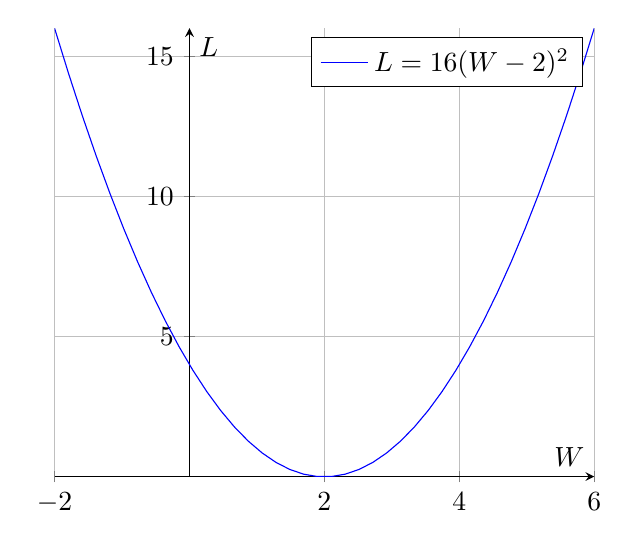
\begin{tikzpicture}
    \begin{axis}[
      axis lines = center,
      xlabel = $W$,
      ylabel = $L$,
      grid = both
    ]
      \addplot[
        domain=-2:6,
        samples=40,
        color=blue
      ]
      {16(x-2)^2}; % function to plot
      \addlegendentry{$L = 16(W-2)^2$}
    \end{axis}
\end{tikzpicture}
\end{center}

We have successfully found the value of W that minimizes the loss. We can do the same for B. In practice, W and B are not constant. They are both variables, and we can vary them together to minimize the loss.

\subsection{Derivative Method}
For simplicity, let us again assume B is constant and set to 0. Now, we are trying to minimize L with respect to W. We can always minimize both of them together, which we will also do shortly.

You may recall from high school calculus that a point where the derivative is equal to 0 corresponds to a minimum or maximum. If the second derivative is positive, it is a minimum. If it is negative, it is a maximum.

Let's calculate the derivative of L with respect to W.
\[
\frac{dL}{dW} = \frac{d}{dW}(16(W-2)^2) \\
\]
\[
= 32(W-2) \\
\]

Setting the derivative to 0, we get:
\[
32(W-2) = 0 \\
\]
\[
32W = 64 \\
\]
\[
W=2 \\
\]

Let's check if it is a maximum or a minimum:

\[
\frac{d^2L}{dW^2} = \frac{d}{dW}(32(W-2)) \\
\]
\[
= 32 \\
\]
Since the second derivative is positive, we have found a minimum.

\subsection{Gradient Calculation}
Although we could use the above method to find the minimum, this process becomes very complex with larger models involving multiple neurons and "layers". It is never used. I only wanted to show you something you were familiar with. We will now use another method called gradient descent.

Gradient descent is a method for finding the minimum of a function by taking small steps in the direction of the negative gradient. The gradient is a vector that points in the direction of the steepest ascent. The negative gradient points in the direction of the steepest descent.

Let me provide an example of how to use gradient descent to find the minimum of a function.

Suppose W was randomly initialized to 0.5. We can calculate the output of the neuron using the formula above. We then calculate the loss L between the output and the ideal output $\hat{Y}$ using the following formula:

\[
Y=WX \\ = 0.5 \cdot 4 \\ = 2 \\
\]
\[
\hat{Y}=8 \\
\]

\[
L = (Y - \hat{Y})^2 \\ = (2 - 8)^2 \\ = 36 \\
\]

The partial derivative of \( Y \) with respect to \( W \) is:

\[
\frac{\partial Y}{\partial W} = \frac{\partial}{\partial W}(WX) = X
\]

Substituting \( X = 4 \):

\[
\frac{\partial Y}{\partial W} = 4
\]

The partial derivative of \( L \) with respect to \( W \) can be found using the chain rule. The chain rule states that if a variable \( z \) depends on \( y \), which in turn depends on \( x \), then the derivative of \( z \) with respect to \( x \) is given by:

\[
\frac{\partial z}{\partial x} = \frac{\partial z}{\partial y} \cdot \frac{\partial y}{\partial x}
\]

Here, \( L \) depends on \( Y \), which in turn depends on \( W \). Using the chain rule:

\[
\frac{\partial L}{\partial W} = \frac{\partial L}{\partial Y} \cdot \frac{\partial Y}{\partial W}
\]

We already know that:

\[
\frac{\partial Y}{\partial W} = X
\]

Now, calculate \( \frac{\partial L}{\partial Y} \):

\[
L = (Y - \hat{Y})^2
\]

\[
\frac{\partial L}{\partial Y} = \frac{\partial}{\partial Y}((Y - \hat{Y})^2) = 2(Y - \hat{Y})
\]

Substituting these into the chain rule:

\[
\frac{\partial L}{\partial W} = \frac{\partial L}{\partial Y} \cdot \frac{\partial Y}{\partial W} = 2(Y - \hat{Y}) \cdot X
\]

Thus, the partial derivative of \( L \) with respect to \( W \) is:

\[
\frac{\partial L}{\partial W} = 2(Y - \hat{Y}) \cdot X
\]

Substituting \( Y = 2 \), \( \hat{Y} = 8 \), and \( X = 4 \):
\[
\frac{\partial L}{\partial W} = 2(2 - 8) \cdot 4 \\
\]
\[
= 2(-6) \cdot 4 \\ = -48 \\
\]

\subsection{Weight Updates}

To reduce the loss, we need to change the value of W in the direction opposite to the gradient. We can do this by subtracting a small fraction of the gradient from W. This fraction is called the learning rate and is denoted by \( \alpha \).

We can update W using the following formula:
\[
W_{new} = W_{old} - \alpha \cdot \frac{\partial L}{\partial W}
\]

Setting \( \alpha = 0.01 \) and substituting the values we have:
\[
W_{new} = 0.5 - 0.01 \cdot (-48) \\
\]
\[
= 0.5 + 0.48 \\ =  0.98 \\
\]
Now, we can repeat the process with the new value of W. I have calculated the values of W, Y, L, and \( \frac{\partial L}{\partial W} \) for the first 20 updates of gradient descent. The results are shown in Table \ref{tab:gradient_descent_iterations}.

\begin{table}[ht]
    \centering
    \begin{tabular}{|c|c|c|c|c|}
        \hline
        Iter & $W$ & $Y$ & $L$ & $\frac{\partial L}{\partial W}$ \\ \hline
         0 & 0.5000 & 2.0000 & 36.0000 & -48.0000 \\ \hline
         1 & 0.9800 & 3.9200 & 16.6464 & -32.6400 \\ \hline
         2 & 1.3064 & 5.2256 & 7.6973 & -22.1952 \\ \hline
         3 & 1.5284 & 6.1134 & 3.5592 & -15.0927 \\ \hline
         4 & 1.6793 & 6.7171 & 1.6458 & -10.2631 \\ \hline
         5 & 1.7819 & 7.1276 & 0.7610 & -6.9789 \\ \hline
         6 & 1.8517 & 7.4068 & 0.3519 & -4.7456 \\ \hline
         7 & 1.8992 & 7.5966 & 0.1627 & -3.2270 \\ \hline
         8 & 1.9314 & 7.7257 & 0.0752 & -2.1944 \\ \hline
         9 & 1.9534 & 7.8135 & 0.0348 & -1.4922 \\ \hline
        10 & 1.9683 & 7.8732 & 0.0161 & -1.0147 \\ \hline
        11 & 1.9784 & 7.9138 & 0.0074 & -0.6900 \\ \hline
        12 & 1.9853 & 7.9414 & 0.0034 & -0.4692 \\ \hline
        13 & 1.9900 & 7.9601 & 0.0016 & -0.3190 \\ \hline
        14 & 1.9932 & 7.9729 & 0.0007 & -0.2170 \\ \hline
        15 & 1.9954 & 7.9816 & 0.0003 & -0.1475 \\ \hline
        16 & 1.9969 & 7.9875 & 0.0002 & -0.1003 \\ \hline
        17 & 1.9979 & 7.9915 & 0.0001 & -0.0682 \\ \hline
        18 & 1.9986 & 7.9942 & 0.0000 & -0.0464 \\ \hline
        19 & 1.9990 & 7.9961 & 0.0000 & -0.0315 \\ \hline
    \end{tabular}
    \caption{Details for the first 20 updates of gradient descent. Note: The loss does not actually become 0; it is just very small and not displayed due to the limited space available.}
    \label{tab:gradient_descent_iterations}
\end{table}

\section{Practical Problems and Concluding Remarks}
\begin{itemize}
    \item The neuron is actually defined as Y = f(WX + B). The function f is a non-linear function. We will discuss why this is necessary in the next lecture. 
    \item We assumed that W=2 and B=0 are ideal values. However, for a single example, W=1 and B=4 is also an ideal solution (as are W=0 and B=8). To generalize for a y=2x function, we will have to provide multiple training examples.
    \item In practice, W and B are varied simultaneously. We can calculate the partial derivative of L with respect to B in a similar way as we did for W.
    Recall $ Y = WX + B $ and $ L = (Y - \hat{Y})^2 $.
    The partial derivative of $ Y $ with respect to $ B $ is:
    \[ \frac{\partial Y}{\partial B} = \frac{\partial}{\partial B}(WX + B) = 1 \]
    Using the chain rule, $ \frac{\partial L}{\partial B} = \frac{\partial L}{\partial Y} \cdot \frac{\partial Y}{\partial B} $. We already know $ \frac{\partial L}{\partial Y} = 2(Y - \hat{Y}) $.
    So,
    \[ \frac{\partial L}{\partial B} = 2(Y - \hat{Y}) \cdot 1 = 2(Y - \hat{Y}) \]
    The update rule for B would then be similar: $ B_{new} = B_{old} - \alpha \cdot \frac{\partial L}{\partial B} $.
    \item All our future work will deal with scaling. Most concepts learned here will continue to be used. We will not be using the derivative method. We will be using the gradient descent method.
    \item Please read AI-11.ipynb to learn how to implement a single neuron network.
\end{itemize}



\end{document}